\documentclass{beamer}
\usepackage[utf8]{inputenc}
\usepackage[english]{babel}
\usepackage{hyperref}
\usepackage{minted}
%%\usemintedstyle{perldoc}
\usetheme{default}
\beamertemplatenavigationsymbolsempty{}

\usepackage{tikz}
\usetikzlibrary{calc,shapes.multipart,chains,arrows}

\title{Implementations of Timing Wheels}
\author{Julian Squires}
\institute{AdGear Technologies, Inc.}
\date{March 16, 2017}
\begin{document}

\begin{frame}
  \titlepage{}
\end{frame}

\begin{frame}{Disclaimers}
  \begin{itemize}
  \item performance claims without benchmarks are damned lies;
  \item I don't understand all these systems;
  \item I'm handwaving on many complex issues, especially concurrency
    and multiprocessor issues.
  \end{itemize}
\end{frame}

\begin{frame}
  Varghese and Lauck. ``Hashed and hierarchical timing
wheels: Data structures for the efficient implementation of a timer
facility.'' ACM SIGOPS Operating Systems Review 21.5 (1987): 25--38.

\vspace{1.5em}

Varghese and Lauck. ``Hashed and hierarchical timing wheels: efficient
data structures for implementing a timer facility.''  IEEE/ACM
transactions on networking 5.6 (1997): 824--834.

\vspace{1.5em}

Varghese. Network Algorithmics: An Interdisciplinary Approach
To Designing Fast Networked Devices. Morgan Kaufmann, 2004.
\end{frame}

\begin{frame}{Recent activity}
  \begin{itemize}
  \item LWN on Gleixner's timing wheels patch:
    \hyperlink{https://lwn.net/Articles/646950/}{https://lwn.net/Articles/646950/}

  \item Adrian Colyer's Morning Paper blog:
    \hyperlink{https://blog.acolyer.org/2015/11/23/hashed-and-hierarchical-timing-wheels/}{https://blog.acolyer.org/2015/11/23/hashed-and-hierarchical-timing-wheels/}

  \item Juho Snellman on Ratas:
    \hyperlink{https://www.snellman.net/blog/archive/2016-07-27-ratas-hierarchical-timer-wheel/}{https://www.snellman.net/blog/archive/2016-07-27-ratas-hierarchical-timer-wheel/}
  \end{itemize}
\end{frame}

\begin{frame}{Timing facility users}
  \begin{columns}[t]
    \column{0.5\textwidth}\centering
    Optimistic\\[.2cm]
    \begin{itemize}
      \item simulations
      \item scheduling
      \item flow control
      \item circuit breakers
      \item watchdogs
    \end{itemize}
    \column{0.5\textwidth}\centering
    Pessimistic\\[.2cm]
    \begin{itemize}
    \item requests awaiting responses
    \item TCP retransmit timers
    \item I/O timeouts
    \end{itemize}
  \end{columns}
\end{frame}

\begin{frame}{Guarantees of a timer system}
  A timer scheduled to fire after $t$ ticks will have its action
  executed, some time after $t$ ticks (if your clock is monotonic and
  doesn't jump forward or skew forward and \ldots)
\end{frame}

\begin{frame}{Design considerations}
  \begin{itemize}
  \item optimistic versus pessimistic
  \item accuracy versus performance
  \item ranged scheduling versus exact
  \item periodic versus one-shot
  \item throughput versus latency
  \item bounded work per timer interrupt
    \begin{itemize}
    \item timer stampede
    \end{itemize}
  \end{itemize}
\end{frame}


\begin{frame}{Unordered lists}
  \begin{center}
    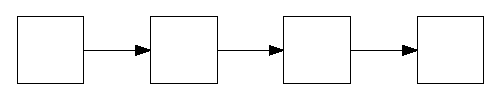
\includegraphics{unordered-list.eps}
  \end{center}
  \begin{itemize}
  \item{Vixie cron}
  \end{itemize}
\end{frame}


%%%% ORDERED LISTS


\begin{frame}{Ordered lists}
  \begin{center}
    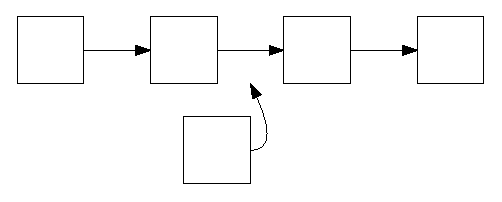
\includegraphics{ordered-list.eps}
  \end{center}

  \begin{itemize}
  \item Zephyr (\hyperlink{http://zephyrproject.org/}{http://zephyrproject.org/})
    \begin{itemize}
    \item \texttt{kernel/include/timeout\_q.h, kernel/timer.c}
    \end{itemize}
  \item XNU (Darwin/macOS) (\hyperlink{http://opensource.apple.com/}{http://opensource.apple.com/})
    \begin{itemize}
    \item \texttt{osfmk/kern/call\_entry.h, osfmk/kern/thread\_call.c, osfmk/kern/timer\_call.c}
    \end{itemize}
  \item pre-1997 Linux, *BSD
  \end{itemize}
\end{frame}


%%%% BINARY HEAPS


\begin{frame}{Binary heaps}
  \hfill 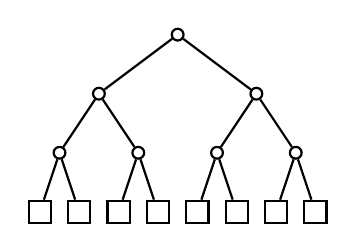
\begin{tikzpicture}
    [-,thick,%
      every node/.style={shape=circle,inner sep=1.5pt,draw,thick},%
      scale=0.5]
    \footnotesize
    \node {}
          [sibling distance=4cm]
          child {node {}
            [sibling distance=2cm]
            child {node {}
              [sibling distance=1cm]
              child {node[rectangle,inner sep=4pt,draw,thick] {}}
              child {node[rectangle,inner sep=4pt,draw,thick] {}}
            }
            child {node {}
              [sibling distance=1cm]
              child {node[rectangle,inner sep=4pt,draw,thick] {}}
              child {node[rectangle,inner sep=4pt,draw,thick] {}}
            }
          }
          child {node {}
            [sibling distance=2cm]
            child {node {}
              [sibling distance=1cm]
              child {node[rectangle,inner sep=4pt,draw,thick] {}}
              child {node[rectangle,inner sep=4pt,draw,thick] {}}
            }
            child {node {}
              [sibling distance=1cm]
              child {node[rectangle,inner sep=4pt,draw,thick] {}}
              child {node[rectangle,inner sep=4pt,draw,thick] {}}
            }
          };
  \end{tikzpicture}

  \vspace{-2em} \begin{itemize}
  \item libev (also a 4-heap!)
  \item libuv
    \begin{itemize}
    \item \texttt{src/heap\_inl.h, src/unix/timer.c}
    \end{itemize}
  \item OpenJDK DelayQueue
    \begin{itemize}
    \item \texttt{src/java.base/share/classes /java/util/concurrent/DelayQueue.java}
    \end{itemize}
  \item Illumos
    \begin{itemize}
    \item \texttt{usr/src/uts/common/os/cyclic.c}
    \item \texttt{usr/src/uts/common/os/callout.c}
    \end{itemize}
  \end{itemize}
\end{frame}


%%%% TIMING WHEELS


\begin{frame}{Timing wheels}
  \begin{center}
    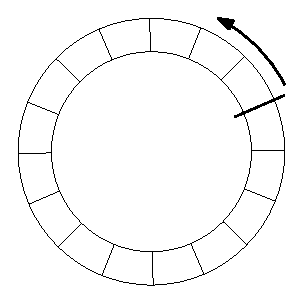
\includegraphics{timing-wheel.eps}
  \end{center}
\end{frame}


%%%% HIERARCHICAL TIMING WHEELS


\begin{frame}{Hierarchical timing wheels}
  \begin{center}
    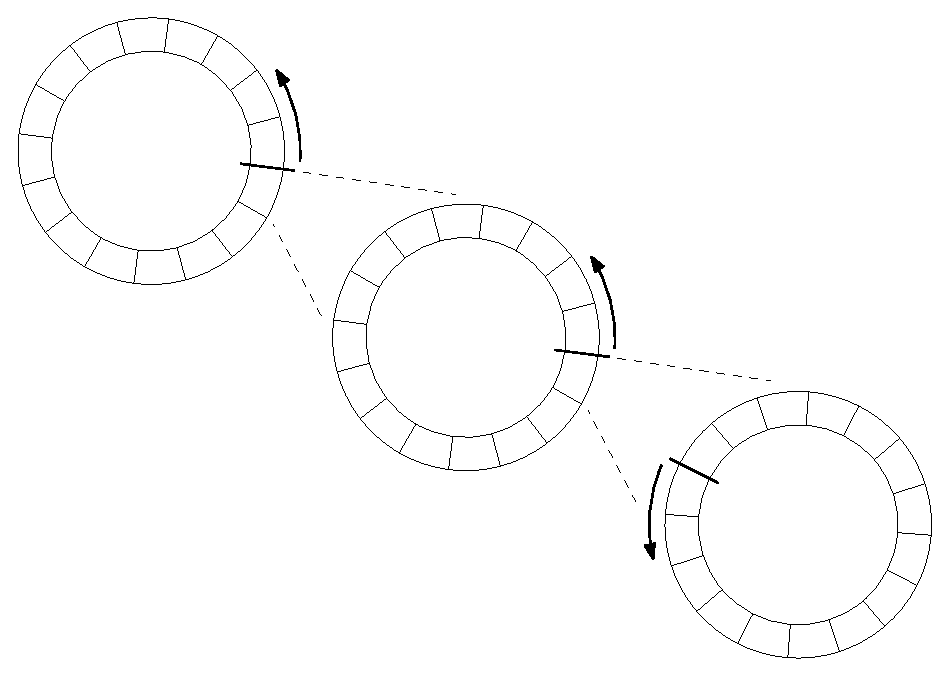
\includegraphics[width=\textwidth]{hierarchical-timing-wheels.eps}
  \end{center}
\end{frame}

\begin{frame}{Hierarchical timing wheels}
  \begin{itemize}
  \item Linux
    \begin{itemize}
    \item \texttt{linux/kernel/time/timer.c}
    \end{itemize}
  \item Ratas (\hyperlink{https://github.com/jsnell/ratas}{https://github.com/jsnell/ratas})
  \item Kafka
    \begin{itemize}
    \item \texttt{core/src/main/scala/kafka/ utils/timer/TimingWheel.scala}
    \end{itemize}
  \item timeout (\hyperlink{https://github.com/wahern/timeout}{https://github.com/wahern/timeout})
  \end{itemize}
\end{frame}


%%%% HASHED TIMING WHEELS


\begin{frame}{Hashed timing wheels}
  \begin{itemize}
  \item *BSD\
    \begin{itemize}
    \item \texttt{sys/kern/kern\_timeout.c}
    \end{itemize}
  \item Erlang (port and proc timers)
    \begin{itemize}
    \item \texttt{erts/emulator/beam/time.c}
    \end{itemize}
  \item Netty
    \begin{itemize}
    \item \texttt{common/src/main/java/io /netty/util/HashedWheelTimer.java}
    \end{itemize}
  \end{itemize}

  \vspace{2em}
  Costello and Varghese. ``Redesigning the BSD callout and timer facilities.'' (1995).
\end{frame}


%%%% OPTIONAL


\begin{frame}{Other techniques}
  \begin{itemize}
  \item calendar queues
  \item skip lists
    \begin{itemize}
    \item DPDK (http://dpdk.org/)
      (\texttt{lib/librte\_timer/rte\_timer.c})
    \end{itemize}
  \item red-black trees
    \begin{itemize}
    \item Linux (\texttt{kernel/time/hrtimer.c})
    \item Erlang (\texttt{erts/emulator/beam/erl\_hl\_timer.c})
    \end{itemize}
  \item hash table
    \begin{itemize}
    \item node.js (\texttt{lib/timers.js})
    \end{itemize}
  \item softheaps?
  \end{itemize}
\end{frame}

\begin{frame}{$O( lg N)$ versus $O(1)$}
Jason Evans says:

\begin{quotation}
In essence, my initial failure was to disregard the difference between
a O(1) algorithm and a O(lg n) algorithm. Intuitively, I think of
logarithmic-time algorithms as fast, but constant factors and large n
can conspire to make logarthmic time not nearly good enough.
\end{quotation}

\hyperlink{http://t-t-travails.blogspot.ca/2008/07/overzealous-use-of-my-red-black-tree.html}{http://t-t-travails.blogspot.ca/2008/07/overzealous-use-of-my-red-black-tree.html}

\end{frame}

\begin{frame}
  
\includegraphics[width=\textwidth]{logo_adgear_smaller.png}
  \\
  \begin{center}
    Julian Squires \\
    \hyperlink{mailto:julian@cipht.net}{$<$julian@cipht.net$>$}
  \end{center}
\end{frame}

\end{document}
